\documentclass[12pt,fleqn]{article}\usepackage{../../common}
\begin{document}
En Yakın k-Komşu (k-Nearest Neighbor), Geometrik Yakınlık Hesabı

Yapay Öğrenim alanında örnek bazlı öğrenen algoritmalardan bilinen KNN, eğitim
verinin kendisini sınıflama (classification) amaçlı olarak kullanır, yeni bir
model ortaya çıkartmaz. Algoritma şöyle işler: etiketleri bilinen eğitim verisi
alınır ve bir kenarda tutulur. Yeni bir veri noktası görülünce bu veriye geri
dönülür ve o noktaya ``en yakın'' k tane nokta bulunur. Daha sonra bu noktaların
etiketlerine bakılır ve çoğunluğun etiketi ne ise, o etiket yeni noktanın
etiketi olarak kabul edilir. Mesela elde \verb!1! kategorisi altında
\verb![2 2]!, \verb!2! kategorisi altında \verb![5 5]!  var ise, yeni nokta
\verb![3, 3]! için yakınlık açısından \verb![2 2]! bulunmalı ve etiket olarak
\verb!1!  sonucu döndürülmelidir.

Üstte tarif edilen basit bir ihtiyaç, yöntem gibi görülebilir. Fakat yapay
öğrenim ve yapay zeka çok boyutlarda örüntü tanıma (pattern recognition)
ile uğraşır, ve milyonlarca satırlık veri, onlarca boyut (üstteki örnekte
2, fakat çoğunlukla çok daha fazla boyut vardır) işler hakikaten
zorlaşabilir. Mesela görüntü tanımada veri \verb!M x N! boyutundaki dijital
imajlar (düzleştirilince $M \cdot N$ boyutunda), ve onların içindeki
resimlerin kime ait olduğu etiket bilgisi olabilir. KNN bu tür multimedya,
çok boyutlu veri ortamında başarılı şekilde çalışabilmektedir. Ayrıca en
yakın k komşunun içeriği tarifsel bilgi çıkarımı (knowledge extraction)
amacıyla da kullanılabilir [2].

``En yakın'' sözü bir kordinat sistemi anlamına geliyor, ve KNN, aynen GMM
ve diğer pek çok kordinatsal öğrenme yöntemi gibi eldeki çok boyutlu veri
noktalarının elemanlarını bir kordinat sistemindeymiş gibi görür. Kıyasla
mesela APriori gibi bir algoritma metin bazlı veriyle olduğu gibi
çalışabilirdi.

Peki arama bağlamında, bir veri öbeği içinden en yakın noktaları bulmanın
en basit yolu nedir? Listeyi baştan sonra taramak (kaba kuvvet yöntemi
-brute force-) listedeki her nokta ile yeni nokta arasındaki mesafeyi teker
teker hesaplayıp en yakın k taneyi içinden seçerdi, bu bir yöntemdir.. Bu
basit algoritmanın yükü $O(N)$'dir. Eğer tek bir nokta arıyor olsaydık,
kabul edilebilir olabilirdi. Fakat genellikle bir sınıflayıcı (classifier)
algoritmasının sürekli işlemesi, mesela bir online site için günde
milyonlarca kez bazı kararları alması gerekebilir. Bu durumda ve $N$'in çok
büyük olduğu şartlarda, üstteki hız bile yeterli olmayacaktır.

Arama işlemini daha hızlı yapmanın yolları var. Akıllı arama algoritmaları
kullanarak eğitim verilerini bir ağaç yapısı üzerinden tarayıp erişim
hızını $O(\log N)$'e indirmek mümkündür.

K-D Ağaçları (k-d tree)

Bilgisayar bilimde K-D ağaçları (k-boyutlu ağaçlar kelimesinin
kısaltılmışı) bir çok boyutlu bölümlere ayırma yaklaşımıdır, eldeki çok
boyutlu veri noktaları bölgelere ayrılarak arama ile bulunmaları
kolaylaştırılmaya uğraşılır. Bu yapı belli bir noktaya en yakın k nokta
bulmaya yardımcı olur.

Yapı şöyledir: K-D ağaçları bir ikisel ağaç olarak kodlanır, ağacın her
düğümü k boyutlu uzayı sadece tek bir kordinat üzerinden ikiye böler. Eğer
3 boyutta isek mesela 1. kordinat üzerinden bu ikiye bölüm
yapılabilir. Ardından o düğümde seçilen kordinat üzerinden bakılan öğeden
daha küçük olan veri noktaları sol dala büyük olanları sağ dala verilir. Bu
işleyiş ağacın altına doğru benzer şekilde devam eder, her seviyede farklı
bir kordinat seçilir.

\inputminted[fontsize=\footnotesize]{python}{kdtree.py}

\begin{minted}[fontsize=\footnotesize]{python}
import bpq, kdtree
tree = kdtree.create([[2,3,4], [4,5,6], [5,3,2]])
print tree.search_nn( (1, 2, 3) )
\end{minted}

\begin{verbatim}
(<KDNode - [2, 3, 4]>, 3.0)
\end{verbatim}

\begin{minted}[fontsize=\footnotesize]{python}
x = np.random.random((1000,2)) * 100.
kx = [list(xxx) for xxx in x]
tree = kdtree.create(kx)
kres = tree.search_knn( [39, 39], k=7 )
for kx in kres: print kx
\end{minted}

\begin{verbatim}
(<KDNode - [37.944809008167091, 36.859556115064997]>, 5.694928053800966)
(<KDNode - [36.282279773622861, 39.25727857203173]>, 7.452195492486094)
(<KDNode - [36.011835939092215, 39.387237685986818]>, 9.07907748034933)
(<KDNode - [38.766178732185438, 34.670053651771802]>, 18.803107763817117)
(<KDNode - [39.443975626797602, 34.581772823651235]>, 19.7178457390171)
(<KDNode - [42.733856969186199, 36.292326352854367]>, 21.27318444578728)
(<KDNode - [43.489959416330848, 37.855783990677935]>, 21.468965836286962)
\end{verbatim}

Küre Agaçları (Ball Tree, BT) 

Bir noktanın diğer noktalara yakın olup olmadığının hesabında yapılması
gereken en pahalı işlem nedir? Mesafe hesabıdır. BT algoritmasının püf
noktası bu hesabı yapmadan, noktalara değil, noktaları kapsayan "kürelere"
bakarak hız kazandırmasıdır. Noktaların her biri yerine o noktaları temsil
eden kürenin pivot noktasına (bu nokta küre içindeki noktaların ortalamasal
olarak merkezi de olabilir, herhangi bir başka nokta da) bakılır, ve oraya
olan mesafeye göre bir küre altındaki noktalara olabilecek en az ve en
fazla uzaklık hemen anlaşılmış olur.

Not: Küre kavramı üç boyutta anlamlı tabii ki, iki boyutta bir çemberden
bahsetmek lazım, daha yüksek boyutlarda ise merkezi ve çapı olan bir
``hiper yüzeyden'' bahsetmek lazım. Tarifi kolaylaştırdığı için çember ve
küre tanımlarını kullanıyoruz.

Mesela elimizde alttaki gibi noktalar var ve küreyi oluşturduk. 

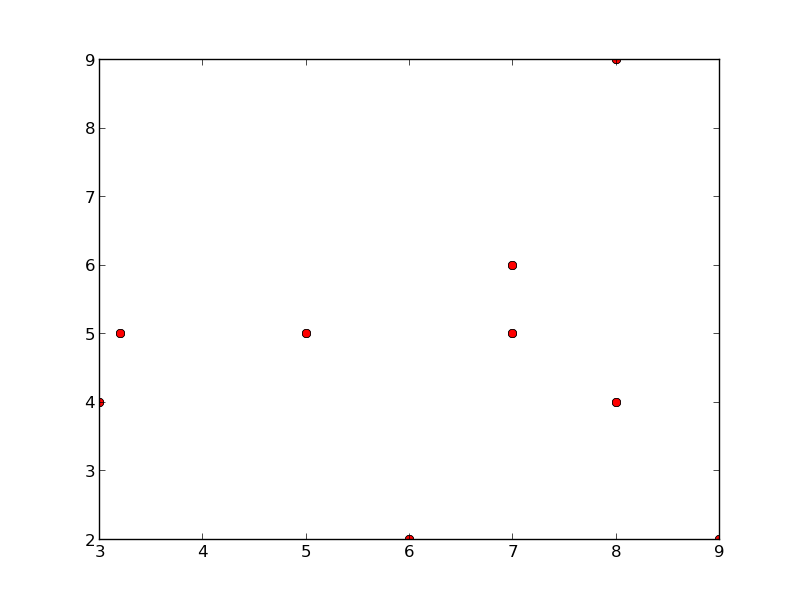
\includegraphics[height=4cm]{knn0.png}

Bu küreyi kullanarak küre dışındaki herhangi bir nokta $q$'nun küredeki
"diğer tüm noktalar $x$'e" olabileceği en az mesafenin ne olacağını
üçgensel eşitsizlik ile anlayabiliriz.

Üçgensel eşitsizlik 

$$ |x-y| \le |x-z| + |z-y| $$

Operatör $|\hspace{0.2cm}|$ norm anlamına gelir ve uzaklık hesabının
genelleştirilmiş halidir. Konu hakkında daha fazla detay {\em Fonksiyonel
  Analiz} ders notlarında. Kısaca söylenmek istenen iki nokta arasında
direk gitmek yerine yolu uzatırsak, mesafenin artacağıdır. Tabii uzaklık,
yol, nokta gibi kavramlar tamamen soyut matematiksel ortamda da işleyecek
şekilde ayarlanmıştır. Mesela mesafe (norm) kavramını değiştirebiliriz,
Öklitsel yerine Manhattan mesafesi kullanırız (blok mesafesi, binalar
etrafından dolaşılıyor, direk gidiş yok), fakat bu kavram bir norm olduğu
ve belirttiğimiz uzayda geçerli olduğu için üçgensel eşitsizlik üzerine
kurulmuş tüm diğer kurallar geçerli olur.

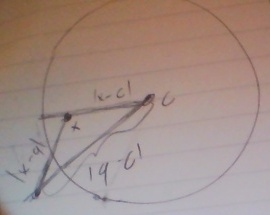
\includegraphics[height=6cm]{tri1.png}

Şimdi diyelim ki dışarıdaki bir $q$ noktasından bir küre içindeki diğer tüm
$x$ noktalarına olan mesafe hakkında bir şeyler söylemek istiyoruz. Üstteki
şekilden bir üçgensel eşitsizlik çıkartabiliriz,

$$ |x-c| + |x-q| \ge |q-c|  $$

Bunun doğru bir ifade olduğunu biliyoruz. Peki şimdi yarıçapı bu işe dahil
edelim, çünkü yarıçap hesabı bir kere yapılıp küre seviyesinde depolanacak
ve bir daha hesaplanması gerekmeyecek, yani algoritmayı hızlandıracak bir
şey olabilir bu, o zaman eğer $|x-c|$ yerine yarıçapı (radius) kullanırsak,
eşitsizlik hala geçerli olur, sol taraf zaten büyüktü, şimdi daha da büyük
olacak, 

$$ radius + |x-q| \ge |q-c|  $$

Bunu nasıl böyle kesin bilebiliyoruz? Çünkü BT algoritması radius'u
$|x-c|$'ten kesinlikle daha büyük olacak şekilde seçer). Şimdi yarıçapı
sağa geçirelim,

$$ |x-q| \ge |q-c| - radius $$

Böylece güzel bir tanım elde ettik. Yeni noktanın küredeki herhangi bir
nokta $x$'e olan uzaklığı, yeni noktanın pivota olan uzaklığının yarıçapı
çıkartılmış halinden {\em muhakkak} fazladır. Yani bu çıkartma işleminden
ele geçen rakam yeni noktanın $x$'e uzaklığına bir "alt sınır (lower
bound)" olarak kabul edilebilir. Diğer tüm mesafeler bu rakamdan daha büyük
olacaktır. Ne elde ettik? Sadece bir yeni nokta, pivot ve yarıçap
kullanarak küredeki "diğer tüm noktalar hakkında" bir irdeleme yapmamız
mümkün olacak. Bu noktalara teker teker bakmamız gerekmeyecek. Bunun nasıl
ise yaradığını algoritma detaylarında göreceğiz.

Benzer şekilde 

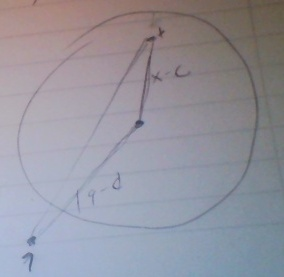
\includegraphics[height=6cm]{tri2.png}

Bu ne diyor? 

$$ |q-c| + |x-c| \ge |q-x| $$

$|x-c|$ yerine yarıçap kullanırsak, sol taraf büyüyeceği için büyüklük hala
büyüklük olarak kalır, 

$$ |q-c| + radius \ge |q-x| $$

Ve yine daha genel ve hızlı hesaplanan bir kural elde ettik (önceki
ifadeye benzemesi için yer düzenlemesi yapalım)

$$ |q-x| \le |q-c| + radius $$

Bu ifade ne diyor? Yeni noktanın pivota olan uzaklığına yarıçap
``eklenirse'' bu uzaklıktan, büyüklükten daha büyük bir yeni nokta / küre
 mesafesi olamaz, küredeki hangi nokta olursa olsun. Bu eşitsizlik te bize
 bir üst sınır (upper bound) vermiş oldu. 

Algoritma \verb!ball_knn!$\left(PS^{in},node\right)$
\begin{enumerate}

\item Eğer alttaki şart geçerli ise node içindeki bir noktanın daha önce
  keşfedilmiş $k$ en yakın komşudan daha yakın olması imkansızdır

\item \verb!if! $D^{node}_{minp} \ge D_{sofar}$ \verb!return!  $PS_{in}$
  değişmemiş halde;

\item \verb!else if! $node$ bir çocuk noktası ise

  \begin{itemize}
   \item  $PS_{out} = PS_{in}$
   \item Her $\forall x \in points(node)$ için
   \begin{itemize}
     \item \verb!if! $\left( |x-q| < D_{sofar} \right)$, basit lineer arama yap
     \item $x$'i $PS_{out}$'a ekle
     \item \verb!if! $|PS^{out}| == k+1$ o zaman en uzak olan komşuyu
       $PS^{out}$'tan çıkart ve $D_{sofar}$'i güncelle
   \end{itemize}

  \end{itemize}

\item Eğer uç nokta değil ise iki çocuk düğümden daha yakın olanını
  incele, sonra daha uzakta olanına bak. büyük bir ihtimalle arama devam
  ettirilirse bu arama kendiliğinden kesilecektir.

  \item \verb!else!
    \begin{itemize}
      \item $node_1 = node$'un $q$'ya en yakın çocuğu;
      \item $node_2 = node$'un $q$'dan en uzak çocuğu;
      \item $PS^{temp} = \verb!ball_knn!(PS^{in},node_1)$;
      \item $PS^{out} = \verb!ball_knn!(PS^{temp},node_2);$
\end{itemize}
        
\end{enumerate}

Küre Ağaçları (BT) metotu önce küreleri, ağaçları oluşturmalıdır. Bu
küreler hiyerarşik şekilde planlanır, tüm noktaların içinde olduğu bir "en
üst küre" vardır her kürenin iki tane çocuk küresi olabilir. Belli bir
(dışarıdan tanımlanan) minimum $r_{min}$ veri noktasına gelinceye kadar
sadece noktaları geometrik olarak kapsamakla görevli küreler oluşturulur,
küreler noktaları sahiplenmezler. Fakat bu $r_{min}$ sayısına erişince
(artık oldukça alttaki) kürelerin üzerine noktalar konacaktır.

Önce tek kürenin oluşturuluşuna bakalım. Bir küre oluşumu için eldeki veri
içinden herhangi bir tanesi pivot olarak kabul edilebilir. Daha sonra bu
pivot'tan diğer tüm noktalara olan uzaklık ölçülür, ve en fazla, en büyük
olan uzaklık yarıçap olarak kabul edilir (her şeyi kapsayabilmesi için).

Not: Bu arada "tüm diğer noktalara bakılması" dedik, bundan kaçınmaya
çalışmıyor muyduk?  Fakat dikkat, "küre oluşturulması" evresindeyiz, k
tane yakın nokta arama evresinde değiliz. Yapmaya çalıştığımız aramaları
hızlandırmak - eğitim / küre oluşturması bir kez yapılacak ve bu eğitilmiş
küreler bir kenarda tutulacak ve sürekli aramalar için ardı ardına
kullanılacaklar.

Küreyi oluşturmanın algoritması şöyledir: verilen noktalar içinde herhangi
birisi pivot olarak seçilir. Sonra bu noktadan en uzakta olan nokta $f_1$,
sonra $f_1$'den en uzakta olan nokta $f_2$ seçilir. Sonra tüm noktalara
teker teker bakılır ve $f_1$'e yakın olanlar bir gruba, $f_2$'ye yakın
olanlar bir gruba ayrılır. 

\begin{minted}[fontsize=\footnotesize]{python}
import balltree, pprint

points = np.array([[3.,3.],[2.,2.]])
q = [1.,1.]
print 'diff', points-q
print 'dist', balltree.dist(points,q)
\end{minted}

\begin{verbatim}
diff [[ 2.  2.]
 [ 1.  1.]]
dist [ 2.82842712  1.41421356]
\end{verbatim}

\inputminted[fontsize=\footnotesize]{python}{balltree.py}

\begin{minted}[fontsize=\footnotesize]{python}
points = np.array([[3.,4.],[5.,5.],[9.,2.],[3.2,5.],[7.,5.],
                 [8.,9.],[7.,6.],[8,4],[6,2]])
tree = balltree.new_node()
balltree.form_tree(points,tree,all_points=points)
pp = pprint.PrettyPrinter(indent=4)
print "tree"
pp.pprint(tree)
newp = np.array([7.,7.])
dummyp = [np.Inf,np.Inf] # it should be removed immediately
res = balltree.search_tree(newp,[np.Inf, [dummyp]], tree, k=2)
print "done", res
\end{minted}

\begin{verbatim}
tree
[   array([ 3.,  4.]),
    7.0710678118654755,
    None,
    [   [   array([ 8.,  9.]),
            3.1622776601683795,
            array([[ 8.,  9.],
       [ 7.,  6.]]),
            [None, None]],
        [   array([ 3.,  4.]),
            6.324555320336759,
            None,
            [   [   array([ 9.,  2.]),
                    3.6055512754639891,
                    None,
                    [   [   array([ 7.,  5.]),
                            1.4142135623730951,
                            array([[ 7.,  5.],
       [ 8.,  4.]]),
                            [None, None]],
                        [   array([ 9.,  2.]),
                            3.0,
                            array([[ 9.,  2.],
       [ 6.,  2.]]),
                            [None, None]]]],
                [   array([ 3.,  4.]),
                    2.2360679774997898,
                    None,
                    [   [   array([ 5.,  5.]),
                            0.0,
                            array([[ 5.,  5.]]),
                            [None, None]],
                        [   array([ 3.,  4.]),
                            1.019803902718557,
                            array([[ 3. ,  4. ],
       [ 3.2,  5. ]]),
                            [None, None]]]]]]]]
None
done [1.0, [[[8.0, 9.0]], [[7.0, 6.0]]]]
\end{verbatim}

Bu iki grup, o anda işlemekte olduğumuz ağaç düğümün (node) iki
çocukları olacaktır. Çocuk noktaları kararlaştırıldıktan sonra artık
sonraki aşamaya geçilir, fonksiyon \verb!form_tree! bu çocuk
noktaları alarak, ayrı ayrı, her çocuk grubu için özyineli (recursive)
olarak kendi kendini çağırır. Kendi kendini çağıran
\verb!form_tree!, tekrar başladığında kendini yeni (bir) nokta
grubu ve yeni bir düğüm objesi ile başbaşa bulur, ve hiçbir şeyden
habersiz olarak işleme koyulur. Tabii her özyineli çağrı yeni düğüm
objesini yaratırken bir referansı üstteki ebeveyn düğüme koymayı
unutmamıştır, böylece özyineli fonksiyon dünyadan habersiz olsa bile,
ağacın en üstünden en altına kesintisiz bir bağlantı zinciri hep
elimizde olur.

Not: \verb!form_tree! içinde bir numara yaptık, tüm noktaların $f_1$'e olan
uzaklığı \verb!dist1!, $f_2$'e olan uzaklığı ise \verb!dist2!. Sonra
\verb!diffs = dist1-dist2! ile bu iki uzaklığı birbirinden çıkartıyoruz ve
mesela \verb!points[diffs <= 0]!  ile $f_1$'e yakın olanları buluyoruz,
çünkü bir tarafta $f_1$'e yakınlık 4 diğer tarafta $f_2$'ye yakınlık 6 ise,
4-6=-2 ie o nokta $f_1$'e yakın demektir. Ufak bir numara ile numpy
dilimleme (slicing) tekniğini kullanabilmiş olduk ve bu önemli çünkü
böylece \verb!for! döngüsü yazmıyoruz, numpy'in arka planda C ile yazılmış
hızlı rutinlerini kullanıyoruz.

Tekrar hatırlatalım: kürelerin sınırları kesişebilir.

Arama 

Üstte sözde program (pseudocode) \verb!ball_knn! olarak gösterilen ve bizim
kodda \verb!search_tree! olarak anılan fonksiyon arama fonksiyonu. Aranan
\verb!new_point!'e olan k en yakın diğer veri noktalar. Dışarıdan verilen
değişken \verb!knn_matches! üzerinde fonksiyon özyineli bir şekilde arama
yaparken "o ana kadar bulunmuş en yakın k nokta" ve o noktaların
\verb!new_point!'e olan en yakın mesafesi saklanır, arama işleyişi
sırasında \verb!knn_matches!, \verb!knn_matches_out! sürekli verilip geri
döndürülen değişkenlerdir, sözde programdaki $P^{in},P^{out}$'un
karşılığıdırlar.

Arama algoritması şöyle işler: şimdi önceden oluşturulmuş küre
hiyerarşisini üstten alta doğru gezmeye başlarız. Her basamakta yeni nokta
ile o kürenin pivot'unu, yarıçapını kullanarak bir "alt sınır mesafe
hesabı" yaparız, bu mesafe hesabının arkasında yatan düşünceyi yazının
başında anlatmıştık. Bu mesafe küre içindeki tüm noktalara olan bir en az
mesafe idi, ve eğer eldeki \verb!knn_matches!  üzerindeki şimdiye kadar
bulunmuş mesafelerin en azından daha az ise, o zaman bu küre "bakmaya
değer" bir küredir, ve arama algoritması bu küreden işleme devam
eder. Şimdiye kadar bulunmuş mesafelerin en azı \verb!knn_matches! veri
yapısı içine \verb!min_so_far!  olarak saklanıyor, sözde programdaki
$D_{sofar}$.

Bu irdeleme sonrası (yani vs küresinden yola devam kararı arkasından)
işleme iki şekilde devam edilebilir, çünkü bir küre iki türden
olabilir; ya nihai en alt kürelerden biridir ve üzerinde gerçek
noktalar depolanmıştır, ya da ara kürelerden biridir (sona gelmedik
ama doğru yoldayız, daha alta inmeye devam), o zaman fonksiyon yine
özyineli bir şekilde bu kürenin çocuklarına bakacaktır - her çocuk
için kendi kendini çağıracaktır. İkinci durumda, kürede noktalar
depolanmıştır, artık basit lineer bir şekilde o tüm noktalara teker
teker bakılır, eldekilerden daha yakın olanı alınır, eldeki liste
şişmeye başlamışsa (k'den daha fazla ise) en büyük noktalardan biri
atılır, vs.

Not: Silme işlemi örnek kodumuzda Python \verb!del! ile
gerçekleştirildi. Eğer bu işlem de hızlandırılmak istenirse, en alt küre
seviyesindeki veriler bir öncelik kuyruğu (priority queue) üzerinde
tutulabilir, ve silme işlemi hep en sondaki elemanı siler, ekleme işlemi
ise yeni elemanı (hep sıralı olan) listede doğru yere koyar.

Daha alta inmemiz gereken birinci durumda yapılan iki çağrının bir
özelliğine dikkat çekmek isterim. Yeni noktanın bu çocuklara olan
uzaklığı da ölçülüyor, ve en önce, en yakın olan çocuğa doğru bir
özyineleme yapılıyor.  Bu nokta çok önemli: niye böyle yapıldı? Çünkü
içinde muhtemelen daha yakın noktaların olabileceği kürelere doğru
gidersek, özyineli çağrıların teker teker bitip yukarı doğru çıkmaya
başlaması ve kaldıkları yerden bu sefer ikinci çocuk çağrılarını
yapmaya başlaması ardından, elimizdeki \verb!knn_matches!
üzerinde en yakın noktaları büyük bir ihtimalle zaten bulmuş
olacağız. Bu durumda ikinci çağrı yapılsa bile tek bir alt sınır
hesabı o kürede dikkate değer hiçbir nokta olamayacağını ortaya
çıkaracak (çünkü en iyiler zaten elimizde), ve ikinci çocuğa olan
çağrılar hiç alta inmeden pat diye geri dönecektir, hiç aşağı
inilmeyecektir.

Bu müthiş bir kazanımdır: zaten bu stratejiye litetürde "budamak (pruning)"
adı veriliyor, bu da çok uygun bir kelime aslında, çünkü ağaçlarla
uğraşıyoruz ve bir düğüm (küre) ve onun altındaki hiçbir alt küreye
uğramaktan kurtularak o dalların tamamını bir nevi "budamış" oluyoruz. Bir
sürü gereksiz işlemden de kurtuluyoruz, ve aramayı hızlandırıyoruz.

Model

KNN'in model kullanmayan, model yerine verinin kendisini kullanan bir
algoritma olarak tanıttık. Peki ``eğitim'' evresi sonrası ele geçen küreler
ve ağaç yapısı bir nevi model olarak görülebilir mi? 

Bu önemli bir soru, ve bir bakıma, evet ağaç yapısı sanki bir modelmiş gibi
duruyor. Fakat, mesela istatistiksel, grafiksel, yapay sınır ağları (neural
net) bağlamında bakılırsa bu yapıya tam bir model denemez. Model bazlı
metotlarda model kurulunca veri atılır, ona bir daha bakılmaz. Fakat KNN,
küre ve ağaç yapısını hala eldeki veriye erişmek için kullanmaktadır. Yani
bir bakıma veriyi ``indeksliyoruz'', ona erişimi kolaylaştırıp
hızlandırıyoruz, ama ondan model çıkartmıyoruz. 

Not: Verilen Python kodu ve algoritma yakın noktaları hesaplıyor sadece,
onların etiketlerinden hareketle yeni noktanın etiketini tahmin etme
aşamasını gerçekleştirmiyor. Fakat bu son aşama işin en basit tarafı,
eğitim veri yapısına eklenecek bir etiket bilgisi ve sınıflama sonrası k
noktanın ağırlıklı etiketinin hesabı ile basit şekilde
gerçekleştirilebilir.

\begin{minted}[fontsize=\footnotesize]{python}
!python plot_circles.py
\end{minted}

Ağaç oluşumu sırasındaki kürelerin grafiği alttadır. 

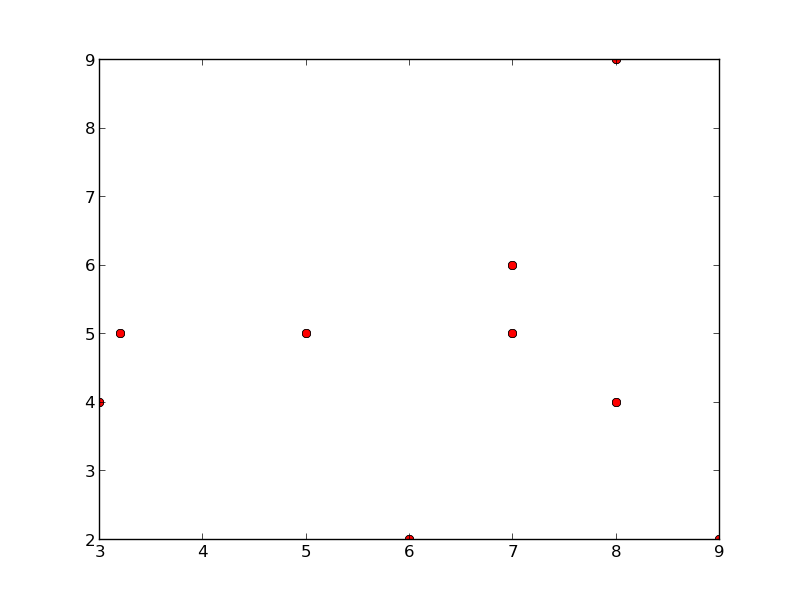
\includegraphics[height=6cm]{knn0.png}
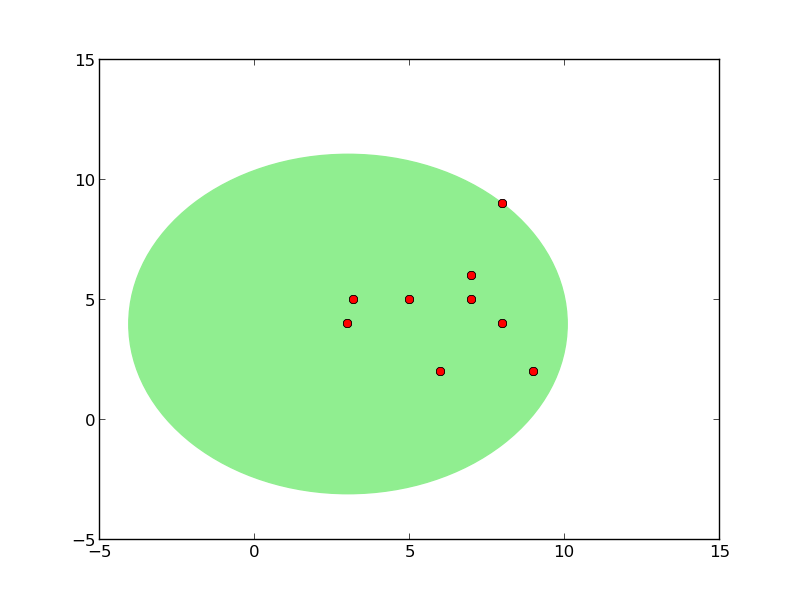
\includegraphics[height=6cm]{knn1.png}
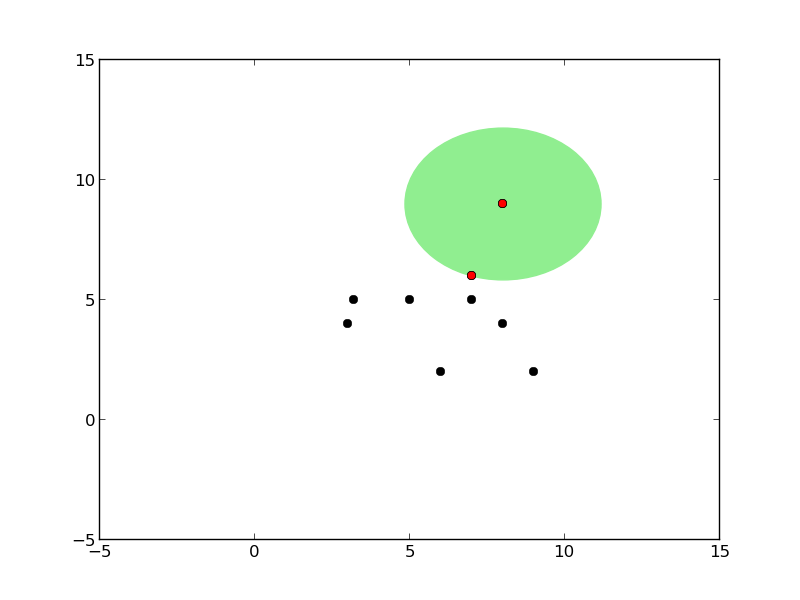
\includegraphics[height=6cm]{knn2.png}
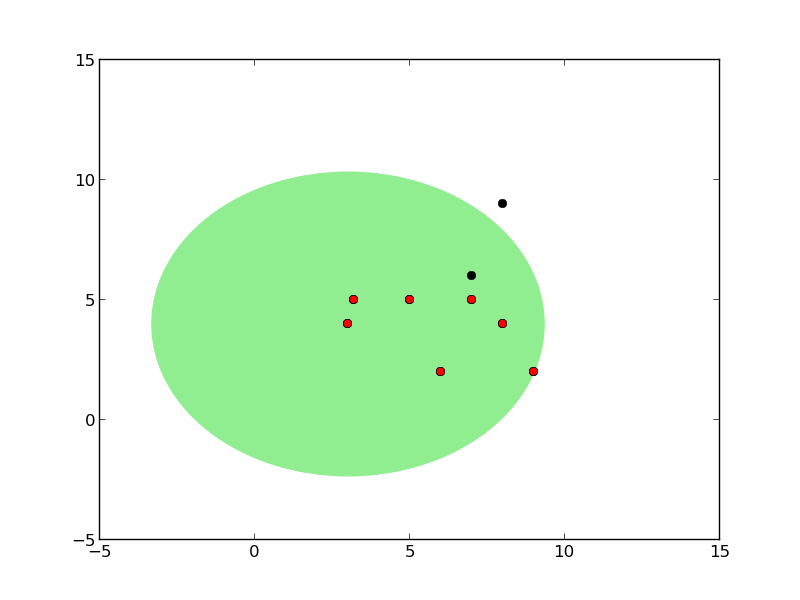
\includegraphics[height=6cm]{knn3.png}
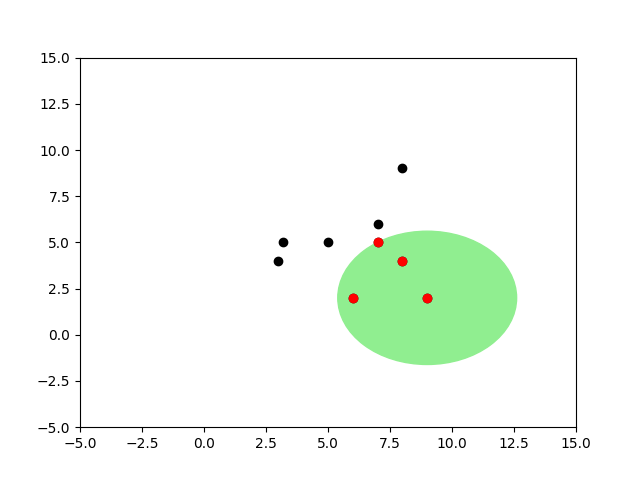
\includegraphics[height=6cm]{knn4.png}
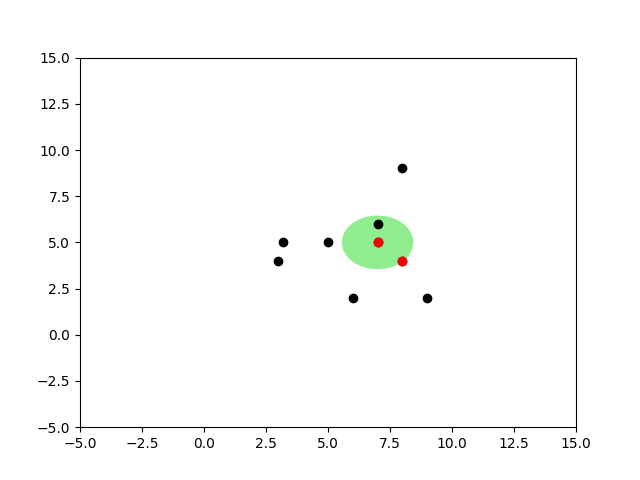
\includegraphics[height=6cm]{knn5.png}
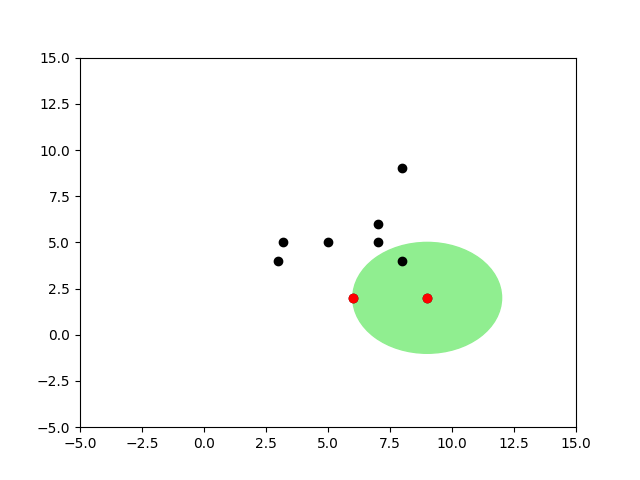
\includegraphics[height=6cm]{knn6.png}
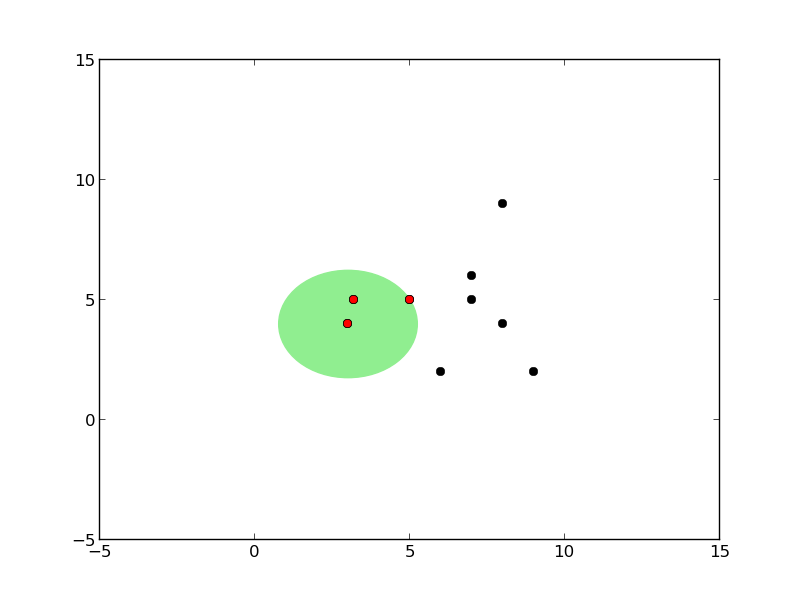
\includegraphics[height=6cm]{knn7.png}
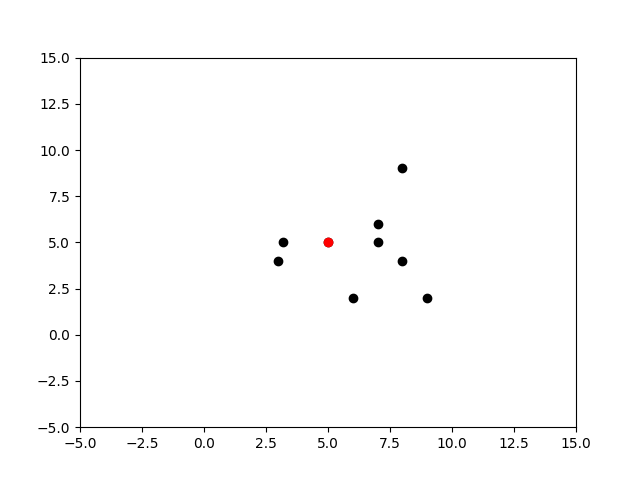
\includegraphics[height=6cm]{knn8.png}
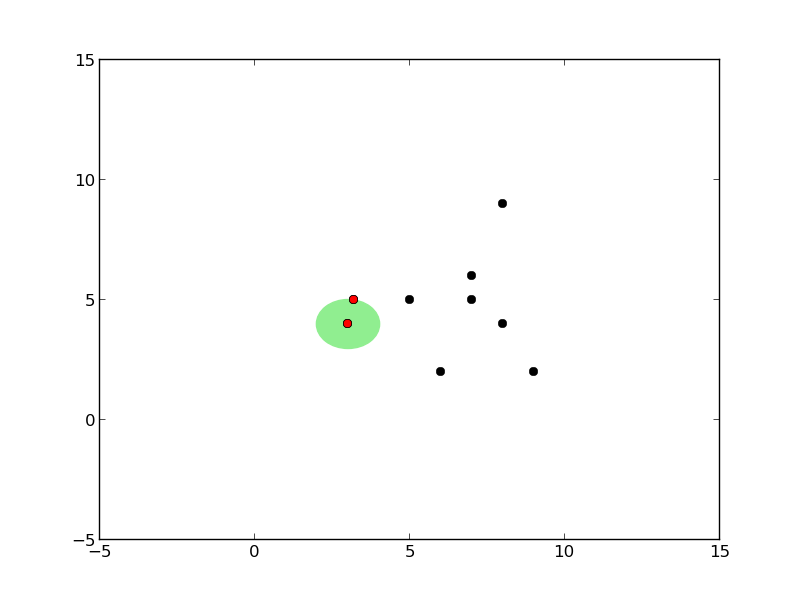
\includegraphics[height=6cm]{knn9.png}

Böleç (Hash) ile Geometrik Anahtarlama

Grafik, fiziksel simülasyonlarda pek çok sayıda obje 3 boyutlu ortamda dünyaya
salınıp, ayrı ayrı onlara fiziksel kurallar uygulanır ve nereye geldiklerine
bakılır. Bu hesap sırasında objelerin birbirine çarpıp çarpmadığını hesaplamak
gerekir fakat böyle bir hesap, eğer mesela $n$ tane obje var ise, her görüntü
karesinde her $n$ tane objenin her $n-1$ diğer objenin yakınında olup olmadığı
kontrolü anlamına gelir, ki hesapsal yük $O(n^2)$ olurdu. Eğer $n$ milyonlar ise
bu ağır bir yük oluştururdu.

Böleç tekniğini burada da kullanabiliriz. Öyle bir sihirli böleç fonksiyonumuz
olsun ki her kordinat için bir böleç değeri üretsin ve birbirine yakın
kordinatlar için bu değer aynı olsun. Böylece basit eşitlik kontrolü ile iki
kordinatın birbirine yakın olup olmadığını hemen anlayabilirdik. Tabii daha
detaylı kontrol için böleçleri aynı olan kordinatları daha detaylı teste tabi
tutardık, ama detaylı kontrolün yapılacağı obje sayısını çok daha azaltmış
olurduk.

Böyle bir tekniği [4]'te görüyoruz. Teknik ile kordinat sistemini $l$
büyüklüğünde kutulara bölüyor, her eksen değerini bu büyüklük ile bölüyoruz,
bölüm sonrası elde edilen sayıyı taban (floor) tamsayıya indirgiyoruz, ardından
her eksen için farklı bir asal sayıyla çarpıp sonuçları XOR ile birleştiriyoruz
(ki XOR yaygın kullanılan bir böleç birleştirme yaklaşımı).

\begin{minted}[fontsize=\footnotesize]{python}
l = 5
n = 5
p1,p2,p3 = 73856093, 19349663, 83492791

x1 = [33,4,11]
x2 = [31,1,14]
x3 = [10,44,19]

def spatial_hash(x):
    ix,iy,iz = np.floor(x[0]/l), np.floor(x[1]/l), np.floor(x[2]/l)
    return (int(ix*p1) ^ int(iy*p2) ^ int(iz*p3)) % n

print (spatial_hash(x1))
print (spatial_hash(x2))
print (spatial_hash(x3))
\end{minted}

\begin{verbatim}
1
1
3
\end{verbatim}

Görüldüğü gibi ilk iki kordinat aynı böleç anahtarına düştü, ki bu iki kordinat
birbirine yakın.

Genel algoritma şöyle olabilir. Her görüntü karesi için iki faz düşünebiliriz,
ilk fazda tüm objelerin kordinat böleci hesaplanır, her böleç değeri altında bir
liste vardır, ve her obje anahtarının değerine tekabül eden o listeye
eklenir. İkinci fazda bir objeye bakarken onun üzerinde daha detaylı çarpışma
hesabı gerekip gerekmediğini anlamak için böleç anahtarındaki listeye bakarız,
listede sadece bir öğe var ise çarpışma yok, birden fazla ise o listedeki her
diğer obje için detaylı çarpışma hesabına devam edilebilir.

Bazi istatistikleri toplayalim. Acaba yaklasim ne kadar basarili?

\begin{minted}[fontsize=\footnotesize]{python}
from collections import defaultdict 
import numpy as np, datetime
import numpy.linalg as lin

mmin,mmax=0,400
p1,p2,p3 = 73856093, 19349663, 83492791
B = 500; L = 50; n = int(B/3)

def spatial_hash(x):
    ix,iy,iz = int(x[0]/L), int(x[1]/L), int(x[2]/L)
    tmp = (ix*p1) ^ (iy*p2) ^ (iz*p3)
    return tmp % n
    
balls = []
geo_hash_list = defaultdict(list)

for b in range(B):
    p = np.array([np.random.uniform(mmin,mmax,1)[0],
                  np.random.uniform(mmin,mmax,1)[0],
                  np.random.uniform(mmin,mmax,1)[0] ])
    balls.append({'pos':p, 'i': b})

for j,b in enumerate(balls):
    geo_hash_list[spatial_hash(b['pos'])].append(b)

tp = 0; tn = 0; fp = 0; fn = 0
for i,b1 in enumerate(balls):
    for j,b2 in enumerate(balls):
        if i==j: continue
        d = lin.norm(b1['pos']-b2['pos'])
        h1 = spatial_hash(b1['pos'])
        h2 = spatial_hash(b2['pos'])
        
        if d <= L and h1 == h2: tp += 1        
        elif d > L and h1 != h2: tn+=1
        elif d > L and h1 == h2: fp+=1
        elif d <= L and h1 != h2: fn+=1

print ('dogru pozitif', tp)
print ('dogru negatif', tn)

print ('yanlis pozitif', fp)
print ('yanlis negatif', fn)

print (tp+tn+fp+fn)
print ("Yanlis Negatif Yuzde %0.2f" % (fn / (tp+tn+fp+fn) * 100.0))
\end{minted}

\begin{verbatim}
dogru pozitif 456
dogru negatif 246340
yanlis pozitif 1340
yanlis negatif 1364
249500
Yanlis Negatif Yuzde 0.55
\end{verbatim}

500 tane topu rasgele bir şekilde her ekseni 0 ve 500 arasında olan bir uzaya
dağıttık. Topların bazıları yakın düştü tabii, bazılar düşmedi. Önce tüm topları
bölecledik ve sözlüğe koyduk. Sonra tüm topların birbiri ile olan mesafesini
ayrı ayrı teker teker külfetli yoldan yaptık, ve bölecin bu durum hakkında ne
söylediğine baktık. Pozitif bölec yakın diyor, negatif bölec uzak diyor
anlamında, tabii yakınlık ve uzaklık bölec anahtar değerinin aynı olup olmadığı
ile ölçülüyor.

Kontrolün doğru pozitif bulması mesela bölecin yakın dediğinin gerçekten de
yakın olması. Yanlış negatif tam tersi, bölec uzak diyor ama aslında toplar
yakın.

Tabii ki istediğimiz doğru hesapların değerlerin yüksek olması. Ayrıca
tekrarlayalım, bir simülasyonda işletirken yanlış pozitifin hala çaresi var,
bölecin yakın dediklerini bir kontrolden daha geçirirsek (problem değil o
noktada bakılan toplar azalmış oluyor, performans kaybı olmaz), bu kontrol
yanlış pozitifleri eleyecektir. Tek problem yanlış negatif, topların çoğu
birbirinden uzakta olduğu için bu yanlıştan dönmek zor, fakat bu tür toplar
yüzde 1'in altında.

C++ bazlı bir kod \verb!CompactNSearch! dizininde. 

Kaynaklar

[1] Liu, Moore, Gray, {\em New Algorithms for Efficient High Dimensional
  Non-parametric Classification}

[2] Alpaydın, {\em Introduction to Machine Learning}

[3] {\em A simple kd-tree in Python}, \url{https://github.com/stefankoegl/kdtree}

[4] {\em Optimized Spatial Hashing for Collision Detection of Deformable Objects}
    \url{https://matthias-research.github.io/pages/publications/tetraederCollision.pdf}


\end{document}




